\chapter{Scripting}

\begin{summary}
This chapter goes deeper into what constitutes a transaction and how scripting is used to lock bitcoins and later unlock them to spend them. Several examples are provided on how to create transactions by calling a node’s API or programmatically.
\end{summary}

\section{Transactions}

A transaction sends bitcoins from one address to another and it consists of 1+ inputs and 1+ outputs. The inputs of a transaction consist of outputs of previous transactions. When an output is spend it can never be used again\footnote{Think of cash. If you give a 20 euro note you can never reuse it. You might be given change but it will be different notes or coins.}. All the bitcoins are transferred elsewhere (to a recipient, back to yourself as change, etc.). Outputs that are available to be spend are called \emph{Unspent Transaction Outputs (UTXOs)} and Bitcoin nodes keep track of the complete UTXO set.

\begin{note}
Each time funds are sent to an address a new output (UTXO) is created. Thus, the balance of an address depends on all the UTXOs that correspond to it. Bitcoin wallets hide UTXOs to make the whole experience friendlier but some wallets allow you to specify which UTXOs you want to spend if needed. When we create transactions programmatically we will deal primarily with UTXOs.
\end{note}

When an output (UTXO) is created we also specify the conditions under which this output can be spend. When you specify an input (the UTXO of a previous transaction) to spend from you have to prove that you satisfy the conditions set by the UTXO.

The spending conditions and the proof that authorizes transfer are not fixed. A scripting language is used to define them. When a new output is created a script is placed in the UTXO called \keyword{scriptPubKey} or more informally locking script.

When we want to spend that UTXO we create a new transaction with an input that references the UTXO that we wish to spend together with an unlocking script or more formally a \keyword{scriptSig}.

The standard transaction output types supported by the Bitcoin protocol are:

\begin{itemize}
\item P2PK (Pay to Public Key - not used anymore)
\item P2PKH (Pay to Public Key Hash)
\item P2SH (Pay to Script Hash)
\item P2WPKH (Pay to Witness Public Key Hash)
\item P2WSH (Pay to Witness Script Hash)
\item OP\_RETURN (allows for storing up to 80 bytes in an output)
\item Multisignature (legacy multisignature transactions; now P2SH/P2WSH is used instead)
\item Non-standard\footnote{Valid Non-standard transactions (containing scripts other than those defined by the standard transaction output type scripts) are rejected and not relayed by nodes. However, they can be mined if it is arranged with a miner.} (any other transaction)
\end{itemize}

The most common transaction output type offering a standard way of transferring bitcoins around is P2PKH (and P2WPKH), which is effectively ``pay to a Bitcoin address''. It is also possible, and used in the past, to pay directly to a public key with P2PK but that is not used anymore. Another very important transaction output type is P2SH (and P2WSH) which allows locking scripts of arbitrary complexity to be used.

To define a locking and unlocking script we make use of a scripting language, simply called \emph{Script}\footnote{https://en.bitcoin.it/wiki/Script}. This relatively simple language consists of several operations each of them identified by an opcode in hexadecimal. It is a simple stack-based language that uses reverse polish notation (e.g. \keyword{2 3 +}) and does not contain potentially dangerous programming constructs, like loops; it is a domain-specific language.

\subsection*{P2PKH}

Let’s examine the standard transaction of spending a Pay to Public Key Hash. The locking script (\keyword{scriptPubKey}) that secures the funds in a P2PKH address is the following:

\begin{emphbox}
\begin{verbatim}
OP_DUP OP_HASH160 <PKHash> OP_EQUALVERIFY OP_CHECKSIG
\end{verbatim}
\end{emphbox}

As we have seen in section \ref{sec:addresses} the public key hash (PKHash) can be derived from the Bitcoin address and vice versa. Thus, the above script locks the funds that have been sent in the address that corresponds to that PKHash.

To spend the funds the owner of the private key that corresponds to that address/PKHash needs to provide an unlocking script that if we prepend to the locking script the whole script will evaluate to true. An unlocking script for a P2PKH will look like this:

\begin{emphbox}
\begin{verbatim}
<Signature> <PublicKey>
\end{verbatim}
\end{emphbox}

% TODO FUTURE SECTION
Using the private key we provide an ECDSA signature of part of the transaction that we create (see future section for more details). We also provide the public key\footnote{As we have already discussed in section~\ref{sec:addresses} the public key only appears in the blockchain after we spend from an address. This is where it appears!} for additional verification.

The validation to spend a UTXO consists of running the script of \keyword{scriptSig} plus \keyword{scriptPubKey}. Both scripts are added in the stack and executed as one script.

\subsection*{Validation of P2PKH Spending}
The validation process is described in below in a step by step explanation during script execution. In each step the script element evaluated will be highlighted (left column) and the current stack (right column) will also be displayed.

%\begin{table}
\begin{center}
\begin{longtable}[H]{ |L{0.47\linewidth}|L{0.47\linewidth}| }
\hline
\multicolumn{2}{|l|}{\emph{Step 0: Execution starts. Stack is empty.}}\\
\hline
\textsf{<Signature> <PublicKey> OP\_DUP OP\_HASH160 <PKHash> OP\_EQUALVERIFY OP\_CHECKSIG} & \\
\hline
\hline
\multicolumn{2}{|l|}{\emph{Step 1: First element is evaluated. It consists of data so it goes into the stack.}} \\
\hline
\textsf{{\color{blue}<Signature>} <PublicKey> OP\_DUP OP\_HASH160 <PKHash> OP\_EQUALVERIFY OP\_CHECKSIG} & \textsf{<Signature>} \\
\hline
\hline
\multicolumn{2}{|l|}{\emph{Step 2: Second element is also data and goes into the stack.}} \\
\hline
\textsf{<Signature> {\color{blue}<PublicKey>} OP\_DUP OP\_HASH160 <PKHash> OP\_EQUALVERIFY OP\_CHECKSIG} & \textsf{<Signature> <PublicKey>} \\
\hline
\hline
\multicolumn{2}{|l|}{\emph{Step 3: Next element is an operator that duplicates the top element of the stack.}}\\
\hline
\textsf{<Signature> <PublicKey> {\color{blue}OP\_DUP} OP\_HASH160 <PKHash> OP\_EQUALVERIFY OP\_CHECKSIG} & \textsf{<Signature> <PublicKey> <PublicKey>} \\
\hline
\hline
\multicolumn{2}{|L{0.94\linewidth}|}{\emph{Step 4: Next element is an operator that calcuates the HASH160 of the top stack element. HASH160 is equivalent to RIPEMD160( SHA256( element ) ) which is what is needed to calculate the PKH from a public key.}}\\
\hline
\textsf{<Signature> <PublicKey> OP\_DUP {\color{blue}OP\_HASH160} <PKHash> OP\_EQUALVERIFY OP\_CHECKSIG} & \textsf{<Signature> <PublicKey> <PKHash>} \\
\hline
\hline
\multicolumn{2}{|L{0.94\linewidth}|}{\emph{Step 5: Next element is data and it is pushed into the stack.}}\\
\hline
\textsf{<Signature> <PublicKey> OP\_DUP OP\_HASH160 {\color{blue}<PKHash>} OP\_EQUALVERIFY OP\_CHECKSIG} & \textsf{<Signature> <PublicKey> <PKHash> <PKHash>} \\
\hline
\hline
\multicolumn{2}{|L{0.94\linewidth}|}{\emph{Step 6: Next element is an operator that checks if the top two elements of the stack are equal and fails the script if they are not. Effectively this validates that the public key provided is indeed the one that corresponds to the PKH (or address) that we are trying to spend.}}\\
\hline
\textsf{<Signature> <PublicKey> OP\_DUP OP\_HASH160 <PKHash> {\color{blue}OP\_EQUALVERIFY} OP\_CHECKSIG} & \textsf{<Signature> <PublicKey>} \\
\hline
\hline
\multicolumn{2}{|L{0.94\linewidth}|}{\emph{Step 7: Next element is an operator that expects two elements from the stack; a signature and a public key that corresponds to that signature. If the signature is valid it returns true, otherwise false.}}\\
\hline
\textsf{<Signature> <PublicKey> OP\_DUP OP\_HASH160 <PKHash> OP\_EQUALVERIFY {\color{blue}OP\_CHECKSIG}} & \textsf{OP\_TRUE} \\
\hline
\end{longtable}
%\caption{Validation steps of P2PKH}
%\label{tab:p2pkh-validation}
\end{center}
%\end{table}

Since the script finished and the only element in the stack is now \keyword{OP\_TRUE}\footnote{Or OP\_1, i.e. true. All the operators, or opcodes, and their explanations can be found at https://en.bitcoin.it/wiki/Script} the node validated ownership of the UTXO and it is allowed to be spent. Success!

To help clarify how addresses, locking scripts and UTXOs relate please see figure~\ref{fig:utxos-pkhashes-addresses}. Addresses 1Zed, 1Alice and 1Bob are short for the actual bitcoin addresses of Zed, Alice and Bob respectively. The diagram emphasises what happens when funds are sent to an address.
\vspace{1em}

\begin{figure}[H]
\begin{center}
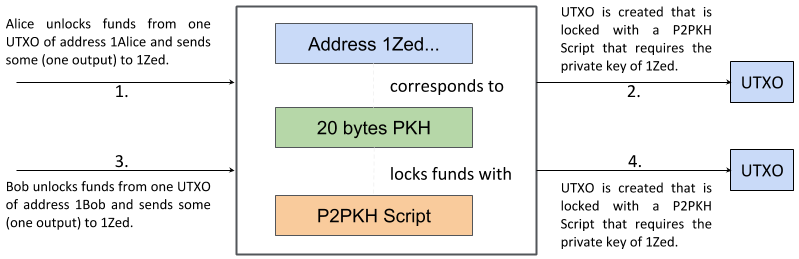
\includegraphics[scale=0.5]{images/utxos-pkhashes-addresses}
\caption{UTXOs, PKHashes and Addresses relationships.}
\label{fig:utxos-pkhashes-addresses}
\end{center}
\end{figure}

This section explained how funds residing in UTXOs are locked/unlocked and how scripts are evaluated for validation. In the next section we will go through several examples of how we can create simple transactions programmatically.

\raggedbottom
